\section{Backtest Results}
\label{sec:backtestresults}

\subsection{Nine-Symbol Paired Benchmark}
\subsubsection{Main class-aware comparison}
Table~\ref{tab:classification} uses all 102 main units, not the 180-point legacy study. Full accuracy is \FullAccuracy\%, Base \BaseAccuracy\%, and CASH/train-majority \CashAccuracy\%. Because 77/102 outcomes are DOWN, ordinary accuracy alone favours conservatism. Full BA is \FullBA\%, Base \BaseBA\%, and logistic-price \LogisticPriceBA\%; the Full--Base BA difference is \DeltaBA\ percentage points. All comparators, including less favourable ones, remain in the table. Undefined constant-rule MCC is NA.

Full and Base each identify seven of 25 UP outcomes. Full issues 24 LONG forecasts, with 17 false positives, versus Base's 29 LONG forecasts and 22 false positives. Thus the observed BA difference accompanies improved DOWN recall rather than additional captured UP cases. This pattern is compatible with a shift towards CASH; it does not identify why the shift occurred or establish information-specific alpha. Neither a higher score than Base nor a smaller loss than an always-invested rule is sufficient evidence of profitability or broad superiority.

Pooled and macro values are different estimands. BHN contributes six eligible units, the other eight symbols twelve; missing class support reduces some macro denominators. Table~\ref{tab:symbol_results} reports Full/Base by symbol. Companion S1 includes all 81 symbol--classifier rows, both-class metrics and all pooled/macro denominators, so comparator reporting is not restricted to selected symbols or the main table's aggregate.
\begin{table}[!htb]
\centering\small
\setlength{\tabcolsep}{3pt}
\renewcommand{\arraystretch}{1.15}
\caption{Class-aware performance on the same 102 historical market units. Macro summaries weight symbols equally and retain undefined denominators.}
\label{tab:classification}
\textbf{A. Pooled (percent except MCC)}\par\smallskip
\begin{tabular}{lrrrrrrrr}
\hline
Strategy & Acc. & BA & MCC & $P_U$ & $R_U$ & $P_D$ & $R_D$ & LONG \\
\hline
Full & 65.69 & 52.96 & 0.060 & 29.17 & 28.00 & 76.92 & 77.92 & 23.53 \\
Base & 60.78 & 49.71 & -0.005 & 24.14 & 28.00 & 75.34 & 71.43 & 28.43 \\
CASH & 75.49 & 50.00 & NA & NA & 0.00 & 75.49 & 100.00 & 0.00 \\
Train-majority & 75.49 & 50.00 & NA & NA & 0.00 & 75.49 & 100.00 & 0.00 \\
Always-LONG & 24.51 & 50.00 & NA & 24.51 & 100.00 & NA & 0.00 & 100.00 \\
Momentum-20 & 49.02 & 47.32 & -0.046 & 22.45 & 44.00 & 73.58 & 50.65 & 48.04 \\
Logistic-price & 67.65 & 55.61 & 0.114 & 33.33 & 32.00 & 78.21 & 79.22 & 23.53 \\
Logistic-matched & 60.78 & 52.42 & 0.044 & 27.27 & 36.00 & 76.81 & 68.83 & 32.35 \\
Factor vote & 51.96 & 51.97 & 0.034 & 26.00 & 52.00 & 76.92 & 51.95 & 49.02 \\
\hline
\end{tabular}\par\medskip
\textbf{B. Unweighted symbol macro summaries}\par\smallskip
\begin{tabular}{lrrrr}
\hline
Strategy & BA (\%) & Defined & MCC & Defined \\
\hline
Full & 55.38 & 8/9 & 0.08 & 8/9 \\
Base & 51.48 & 8/9 & 0.00 & 8/9 \\
CASH & 50.00 & 8/9 & NA & 0/9 \\
Train-majority & 50.00 & 8/9 & NA & 0/9 \\
Always-LONG & 50.00 & 8/9 & NA & 0/9 \\
Momentum-20 & 50.67 & 8/9 & -0.01 & 8/9 \\
Logistic-price & 59.00 & 8/9 & 0.17 & 7/9 \\
Logistic-matched & 56.55 & 8/9 & 0.08 & 8/9 \\
Factor vote & 46.86 & 8/9 & -0.04 & 8/9 \\
\hline
\end{tabular}\par\medskip
\begin{minipage}{\textwidth}\footnotesize $N=102$, UP/DOWN=25/77. P/R denote class precision/recall. NA is undefined, including MCC for constant predictions. Train-majority is fit on purged train labels. Logistic-matched uses common numerical market inputs, not identical chart/text representations. Full per-symbol/class metrics are supplied in companion S1; hold has no classification prediction.\end{minipage}
\end{table}


\subsubsection{Account outcomes and exposure}
Full mean net account return is \FullReturn\%, versus Base \BaseReturn\% and CASH zero (Table~\ref{tab:accounts}). Full therefore does not even outperform Base on this main economic mean, despite its higher BA. Always-LONG cycles and continuous hold have different costs and gap exposure, and neither is substituted for the other. The held-session fractions include the long CASH gaps between the two cutoffs in each block; their low values should not be confused with LONG percentages over scheduled decision units.

Returns and drawdowns summarize separate accounts, not one portfolio, total-return index or certified executable strategy. Risk ratios cannot recover evidence of profitability from sparse trades. The main schedules have 57 observed sessions between cutoffs, so pending-cash/on-demand-advance equivalence on these accounts provides little evidence about rapid capital reuse. All twelve economic sensitivities are reported in Table~\ref{tab:execution}. The all-entries-missed scenario gives zero but is not a mathematical worst-return bound; other assumptions may introduce unfilled entries, delays, pending balances or residual shares. Predictions and classification labels are unchanged across these sensitivities.
\begin{table}[!htb]
\centering\small
\setlength{\tabcolsep}{3pt}
\renewcommand{\arraystretch}{1.15}
\caption{Account outcomes under the fractional reference ledger. Means summarize 51 separate symbol–block accounts per strategy and do not establish executable portfolio returns.}
\label{tab:accounts}
\textbf{Reference ledger}\par\smallskip
\begin{tabular}{lrrrr}
\hline
Strategy & Return (\%) & MDD (\%) & Held (\%) & Orders \\
\hline
Full & -0.797 & 1.37 & 2.35 & 0.94 \\
Base & -0.750 & 1.45 & 2.84 & 1.14 \\
CASH & 0.000 & 0.00 & 0.00 & 0.00 \\
Train-majority & 0.000 & 0.00 & 0.00 & 0.00 \\
Always-LONG & -3.000 & 4.52 & 10.00 & 4.00 \\
Momentum-20 & -1.636 & 2.58 & 4.80 & 1.92 \\
Logistic-price & -0.683 & 1.18 & 2.35 & 0.94 \\
Logistic-matched & -1.105 & 1.60 & 3.24 & 1.29 \\
Factor vote & -1.457 & 2.49 & 4.90 & 1.96 \\
Continuous hold & -2.127 & 12.94 & 100.00 & 2.00 \\
\hline
\end{tabular}\par\medskip
\begin{minipage}{\textwidth}\footnotesize Each row averages 51 independent-capital symbol--block accounts, not a portfolio. Held is the fraction of observed calendar sessions held, including scheduled CASH gaps; it differs from the LONG rate. Continuous hold buys once and sells once across gaps. Dividends/corporate actions and fills are not certified. Annualised cycle Sharpe/Sortino are omitted for irregular/gapped schedules.\end{minipage}
\end{table}


\subsubsection{Separate extension comparison on the shared calendar}
Table~\ref{tab:u09-comparison} reports all ten extension roles/controls, retaining both baselines and every bypass. Native mean account return is \UnifiedNativeReturn\%, Common \UnifiedCommonReturn\%, Bayesian v1 \UnifiedVOneReturn\% and MT-BICL \UnifiedMTReturn\%. Their BAs are \UnifiedNativeBA\%, \UnifiedCommonBA\%, \UnifiedVOneBA\% and \UnifiedMTBA\%, respectively. These are U09 outcomes, not replacements for the original Full/Base numbers above. Every research role's mean account return is negative, whereas CASH is zero; Always-LONG cycles return \UnifiedAlwaysLongReturn\% under the same two-leg costs.

Bayesian v1 minus Common has mean return difference $+\UnifiedVOneCommonReturnEffect$ pp with descriptive simultaneous band $[\UnifiedVOneCommonReturnLow,\UnifiedVOneCommonReturnHigh]$. Against Native, its difference is $\UnifiedVOneNativeReturnEffect$ pp with band $[\UnifiedVOneNativeReturnLow,\UnifiedVOneNativeReturnHigh]$. The comparator therefore changes the interpretation: the recorded improvement over Common does not establish an advantage over the native system. MT-BICL minus Native is $\UnifiedMTNativeReturnEffect$ pp with band $[\UnifiedMTNativeReturnLow,\UnifiedMTNativeReturnHigh]$; the negative result is retained. Full precision and all twenty return/BA contrasts are reported in \ref{app:additional} and the source companions, not recomputed from rounded table cells.
% Giữ bảng chính gần phần diễn giải và trước figure; không sửa artifact generated đã khóa.
\begingroup
\let\savedcomparisontable\table
\def\table[#1]{\savedcomparisontable[!htbp]}
\begin{table}[htb]
\centering\small
\setlength{\tabcolsep}{3pt}
\renewcommand{\arraystretch}{1.12}
\caption{Mean returns, balanced accuracy and support across historical-context methods and controls.}
\label{tab:u09-comparison}
\textbf{Paired support: 102 points per repeat}\par\smallskip
\begin{tabular}{lrrrrrr}
\hline
Role & Return (\%) & BA (\%) & LONG (\%) & Raw & Bypass & $N$/repeat \\
\hline
Native & -0.653 & 51.84 & 22.55 & 306 & 0 & 102 \\
Common & -1.025 & 45.97 & 28.76 & 306 & 0 & 102 \\
Bayesian & -0.698 & 50.10 & 23.86 & 144 & 162 & 102 \\
Conditional & -1.030 & 45.75 & 29.08 & 3 & 303 & 102 \\
Trend--pattern & -1.019 & 46.18 & 28.43 & 24 & 282 & 102 \\
Explicit counts & -1.030 & 45.75 & 29.08 & 3 & 303 & 102 \\
MT-BICL & -1.253 & 43.17 & 34.31 & 198 & 108 & 102 \\
Fact anchor & -1.286 & 42.74 & 34.97 & 306 & 0 & 102 \\
CASH & 0.000 & 50.00 & 0.00 & 0 & 306 & 102 \\
Always-LONG & -3.000 & 50.00 & 100.00 & 0 & 306 & 102 \\
\hline
\end{tabular}\par\medskip
\begin{minipage}{\textwidth}\footnotesize Return averages 51 accounts after averaging three repeats; BA averages per-repeat metrics, and Raw/Bypass counts cover 306 method slots.\end{minipage}
\end{table}

\endgroup
\FloatBarrier

Figure~\ref{fig:u09-return-contrasts} displays all five extension-versus-baseline return differences for each baseline. The panels use the same frozen analysis and simultaneous family as the tabulated contrasts; changing the displayed baseline does not create another experiment.
\begin{figure}[!htbp]
\centering
% Chỉ cắt khung hiển thị hai panel từ cùng PNG 1692x666, 180 dpi; không sửa byte ảnh/số liệu.
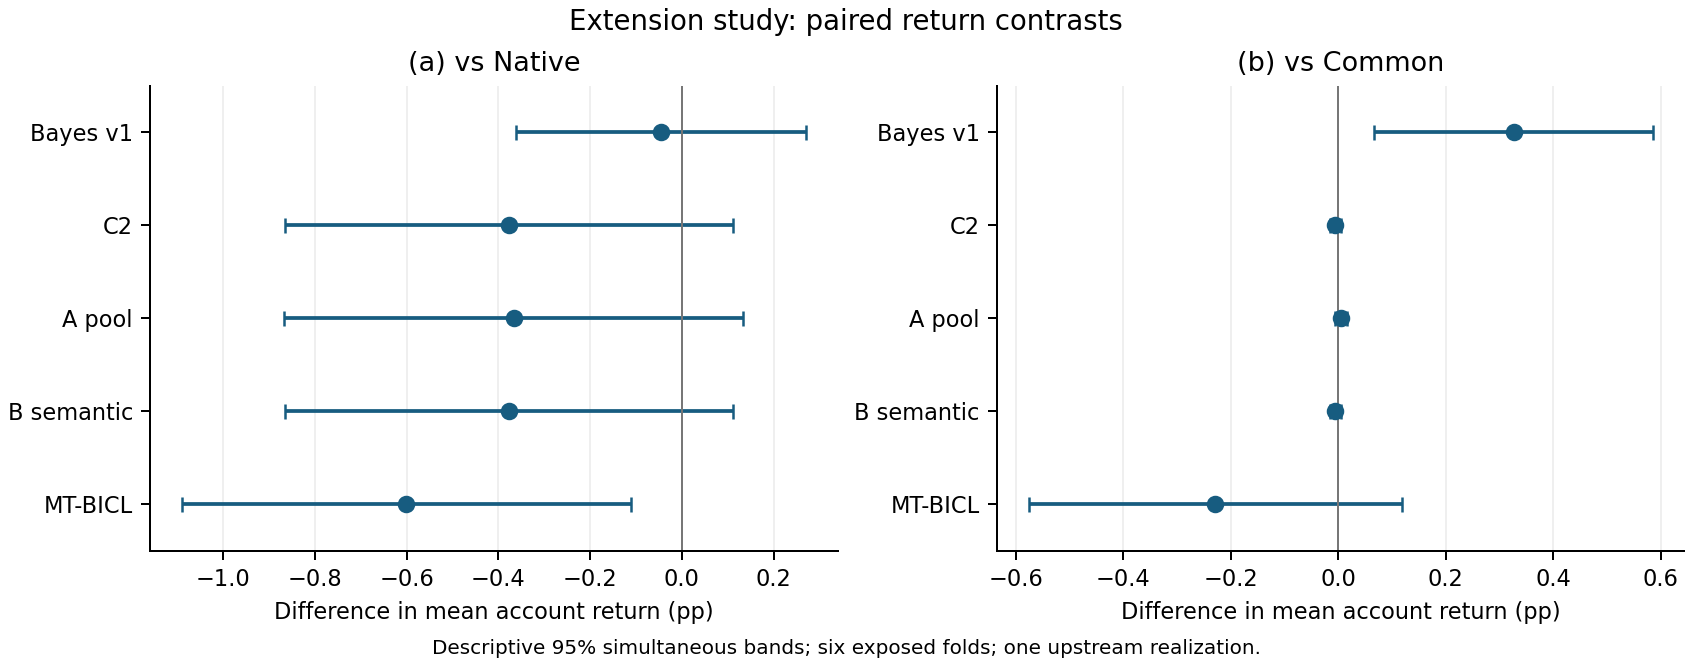
\includegraphics[width=0.78\textwidth,trim=0bp 14.4bp 336.8bp 18bp,clip]{generated/u09/return_contrasts.png}\par\smallskip
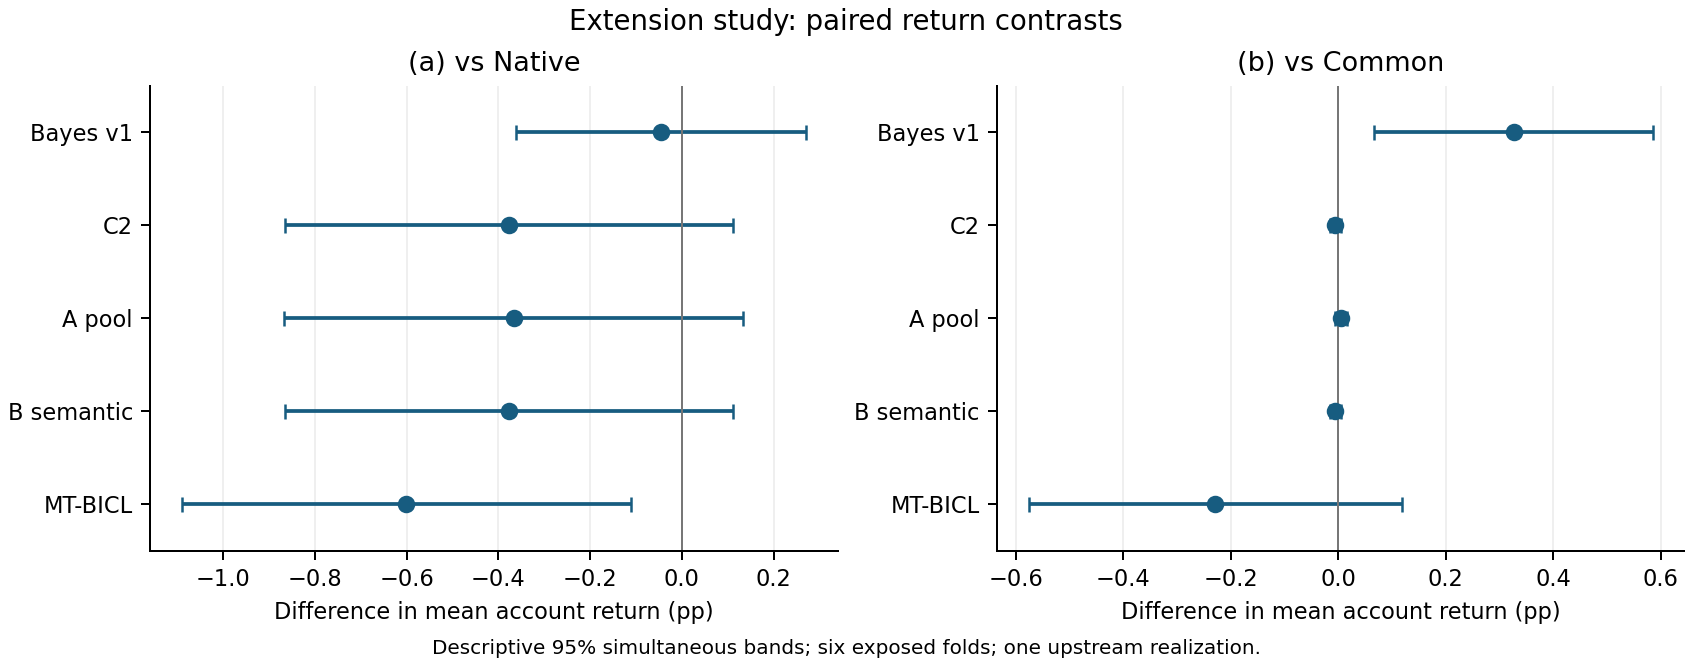
\includegraphics[width=0.78\textwidth,trim=340bp 14.4bp 0bp 18bp,clip]{generated/u09/return_contrasts.png}
\caption{Extension mean account-return contrasts against Native (top) and Common (bottom), in percentage points. The frozen two-panel image is displayed as enlarged panels with separate horizontal scales. Points and descriptive 95\% simultaneous bands come from the paired circular-fold bootstrap (10,000 draws, primary block length L2; joint family of twenty return/BA contrasts). The vertical line denotes zero difference. Bands describe sensitivity on six exposed folds, not calibrated significance or deployable profitability. Both panels retain every extension, including adverse results; uncertainty is conditional on one upstream realization.}
\label{fig:u09-return-contrasts}
\end{figure}

Coverage is part of these method outcomes. C2 and B\_semantic each have only \UnifiedCTwoRaw\ raw Decisions and \UnifiedCTwoBypass\ bypasses per 306 slots; A\_tp\_pool has \UnifiedAPoolRaw\ raw Decisions, Bayesian v1 \UnifiedVOneRaw\ and MT-BICL \UnifiedMTRaw. A fallback reuses the same repeat's parent action and is included in primary metrics, not removed as a failed observation. Table~\ref{tab:u09-support} separates CORE4/OOD5 and recorded effective K; \UnifiedMissingSentiment/\UnifiedPoints\ points have unavailable sentiment. Consequently, near-equal outcomes of C2/B and Common primarily reflect coverage and policy, not evidence that the corresponding retrievers extracted equivalent useful information.

\subsection{Disentangled Alpha--Sentiment Ablation}
\subsubsection{Repeated executions and factorial contrasts}
Table~\ref{tab:repeats} retains all three executions, sample SD, range and cutoff-level prediction disagreement summaries. The two panels have nine market units each but different symbols, dates and prompt families. Their means and SDs are not transferable to the broad 102-unit main study. Zero metric SD does not imply identical predictions: factorial S has unchanged aggregate BA but nonzero disagreement. Return means use nine upstream or eight factorial symbol--block accounts per variant/execution.

On the factorial panel the AS--B BA mean is $-9.52$ pp and AS--P is $-11.90$ pp. Interaction $AS-A-S+B$ is $+14.29$ pp, whereas the gap of mean BA between AS and the observed best single component is zero. These are different quantities. All seven descriptive BA family envelopes contain zero; only 6,986 of 10,000 BA draws retain both classes and 3,014 are undefined. Conditional intervals are not zero-imputed or advertised as calibrated familywise coverage. All factorial mean account returns are negative.

The upstream AS--B mean BA difference is $+4.76$ pp, with conditional percentile interval $[0,10]$ pp. This higher-performing small panel does not replace the main or factorial outcomes. Actual shared reports and paired prompt contents match their frozen parents, but 40 of 147 groups have a successful-call order different from the listed job order, and nine span execution epochs. Routing/quota/resume did not implement full counterbalancing. We retain every outcome and disclose the resulting time/order confounding rather than selecting a clean-looking subset or repairing it retrospectively.
\begin{table}[htb]
\centering\small
\setlength{\tabcolsep}{3pt}
\renewcommand{\arraystretch}{1.15}
\caption{Prediction variability and paired contrasts across three executions of two nine-observation panels.}
\label{tab:repeats}
\textbf{A. Three executions: mean (sample SD)}\par\smallskip
\begin{tabular}{lrrrrr}
\hline
Panel/variant & Acc. (\%) & BA (\%) & BA range & Disagr. (\%) & Return (\%) \\
\hline
U B & 85.19 (16.97) & 90.48 (10.91) & [78.57, 100.00] & 22.22 & 0.37 (0.38) \\
U AS & 92.59 (6.42) & 95.24 (4.12) & [92.86, 100.00] & 7.41 & 0.50 (0.22) \\
F B & 44.44 (11.11) & 28.57 (7.14) & [21.43, 35.71] & 14.81 & -1.70 (0.55) \\
F A & 29.63 (6.42) & 19.05 (4.12) & [14.29, 21.43] & 22.22 & -2.03 (0.31) \\
F S & 22.22 (0.00) & 14.29 (0.00) & [14.29, 14.29] & 22.22 & -2.34 (0.22) \\
F AS & 29.63 (16.97) & 19.05 (10.91) & [7.14, 28.57] & 22.22 & -2.23 (0.63) \\
F P & 48.15 (6.42) & 30.95 (4.12) & [28.57, 35.71] & 14.81 & -1.42 (0.33) \\
\hline
\end{tabular}\par\medskip
\textbf{B. BA contrasts in percentage points}\par\smallskip
\begin{tabular}{lrrrrr}
\hline
Contrast & Mean & SD & Range & Percentile & Family env. \\
\hline
U AS-B & 4.76 & 8.25 & [0.00, 14.29] & [0.00, 10.00] & NA \\
F AS-B & -9.52 & 10.91 & [-21.43, 0.00] & [-22.22, 9.52] & [-37.14, 18.10] \\
F A-B & -9.52 & 4.12 & [-14.29, -7.14] & [-20.37, 14.29] & [-37.14, 18.10] \\
F AS-S & 4.76 & 10.91 & [-7.14, 14.29] & [-6.67, 24.07] & [-22.86, 32.38] \\
F S-B & -14.29 & 7.14 & [-21.43, -7.14] & [-29.63, 10.00] & [-41.90, 13.33] \\
F AS-A & 0.00 & 12.37 & [-14.29, 7.14] & [-20.00, 11.11] & [-27.62, 27.62] \\
F AS-P & -11.90 & 14.87 & [-28.57, 0.00] & [-28.57, 4.76] & [-39.52, 15.71] \\
F interaction & 14.29 & 14.29 & [0.00, 28.57] & [-16.67, 38.89] & [-13.33, 41.90] \\
\hline
\end{tabular}\par\medskip
\begin{minipage}{\textwidth}\footnotesize U/F denote upstream/factorial panels; BA intervals condition on 6,986 finite draws, with 3,014 undefined draws among 10,000 resamples.\end{minipage}
\end{table}


\subsubsection{Extension bridges do not replace missing ablations}
Table~\ref{tab:u09-bridge} distinguishes the native-to-common alpha/prompt bridge, the fact-anchor bridge and the MT revision step. MT agrees with Fact\_Anchor on 302/306 final actions. This limits attribution of the total MT-versus-baseline outcome to the numerical student or retrieved context. The earlier alpha/sentiment/placebo panels remain separate evidence; U09 did not execute retrieval-only, statistics-only, no-prior, no-target or no-utility interventions. Registry support for an ablation is not an observed result. A controlled component study would require its own protocol and executions.

\subsection{Robustness and Sensitivity}
\subsubsection{Temporal and dependence diagnostics}
Table~\ref{tab:temporal} keeps the all-102 primary cohort and two overlapping structural cohorts. The primary Full--Base BA interval is $[\PrimaryLow,\PrimaryHigh]$ pp. The common-eight cohort has 96 units over twelve dates; recent-nine has 54 over six dates. They are sensitivity views, not independent replications or grounds for choosing a more favourable headline. The six-block sample includes an all-DOWN early-2025 block: within-block BA without both classes is undefined rather than fabricated.

Past Close/SMA60 contexts distinguish bull, bear and sideways observations. These are per-security descriptions, not validated market-wide index regimes or a regime-conditioned trading policy. Additional volatility and turnover-proxy thresholds are fitted on purged training data, but their post-inference stratification remains descriptive. Close times Volume is in vendor units, not measured spread/depth liquidity. Exposure based on three target sessions differs from whole-calendar exposure with gaps.

Calendar-aligned HAC accuracy effects for common-eight/recent-nine are $+3.125/+9.259$ pp. At lags 0/1/2, common-eight SEs are 0.026042/0.023146/0.020172 with $p$-values 0.255346, 0.204107 and 0.149610; recent-nine SEs are 0.040713/0.047112/0.045710 with $p$-values 0.072051, 0.106554 and 0.098654. These are accuracy, not BA, effects on twelve/six selected dates. Companion S4 retains all six rows, the calendar masks, all regime strata, block-length sensitivities and leave-one-block-out diagnostics. Few clusters and irregular dates prevent reliable significance, null-effect or calibrated-coverage conclusions.
\begin{table}[!htb]
\centering\small
\setlength{\tabcolsep}{3pt}
\renewcommand{\arraystretch}{1.15}
\caption{Overlapping temporal cohorts and observed trend strata. Small-block intervals and calendar-aligned HAC diagnostics are descriptive rather than calibrated significance tests.}
\label{tab:temporal}
\textbf{A. Cohorts: BA percent; difference/interval in pp}\par\smallskip
\begin{tabular}{lrrrrrrr}
\hline
Cohort & $N$ & Dates & Blocks & Full & Base & $\Delta$ & Interval \\
\hline
All & 102 & 12 & 6 & 52.96 & 49.71 & 3.25 & [-1.18, 8.13] \\
Common eight & 96 & 12 & 6 & 50.69 & 48.61 & 2.08 & [-1.20, 5.26] \\
Recent nine & 54 & 6 & 3 & 53.08 & 46.67 & 6.41 & [0.00, 12.50] \\
\hline
\end{tabular}\par\medskip
\textbf{B. Observed per-security trend contexts (percent)}\par\smallskip
\begin{tabular}{lrrrrrr}
\hline
Trend & $N$ & UP/DOWN & Full BA & Base BA & Full LONG & Base LONG \\
\hline
Bear & 35 & 5/30 & 43.33 & 41.67 & 11.43 & 14.29 \\
Bull & 33 & 9/24 & 47.92 & 53.47 & 36.36 & 39.39 \\
Sideways & 34 & 11/23 & 59.49 & 46.25 & 23.53 & 32.35 \\
\hline
\end{tabular}\par\medskip
\begin{minipage}{\textwidth}\footnotesize Cohorts overlap and are not pooled as extra samples. Trend uses past Close/SMA60 with strict +/-2\% thresholds; it is not an index-regime policy. Primary intervals retain both dates, full cross-sections and pairing within blocks. HAC concerns accuracy rather than BA and is reported for both fixed-universe panels at lags 0/1/2 in S4.\end{minipage}
\end{table}


\subsubsection{Auxiliary numeric selector controls}
Table~\ref{tab:numeric} is a separate numeric study, not an LLM factor-selector ablation. Causal adapters and train-only eligibility, imputation, scaling, orientation and ranking are fitted once per symbol--block scope, then retained through validation/test. Fixed custom five, dynamic train top-five, the same IDs without sign flip, and all twenty random eligible-five trials produce 2,346 predictions on the same 102 units. No random seed is selected after observing results.

Dynamic-minus-fixed, dynamic-minus-random-family and dynamic-minus-no-flip BA differences are respectively $+15.84$, $+7.33$ and $+6.44$ pp. Exact six-block two-sided sign-flip values are 0.0625, 0.125 and 0.53125; Holm correction \cite{holm1979multiple} over all 23 declared hypotheses gives adjusted $p=1$ throughout. Unadjusted percentile intervals and the entire random dispersion remain visible. Positive point differences do not establish superiority, and the no-flip contrast does not identify sign-flip value inside the LLM pipeline.

Native diagnostics separately account for 102 cutoffs, 8,670 candidate opportunities and 510 selected slots. WQ42 occurs at 52/102 cutoffs (52/510 slots); adjacent nonzero IC signs flip 1,282 times over 7,894 eligible transition pairs. These are dependent in-sample diagnostics, not out-of-sample alpha stability. Complete per-factor frequency, eligible denominators, IC signs, windows and all 21 exclusions are retained in the registry companion. Numeric controls do not repair native row-wise noncausality, provide the missing fixed/random LLM experiment, or certify original-expression equivalence.
\begin{table}[!htb]
\centering\small
\setlength{\tabcolsep}{3pt}
\renewcommand{\arraystretch}{1.15}
\caption{Train-fit numeric selector controls using separate causal adapters. These auxiliary results neither repeat the native LLM selector experiment nor repair its row-wise causal defect.}
\label{tab:numeric}
\textbf{A. Pooled numeric results; random mean (SD)}\par\smallskip
\begin{tabular}{lrrrrr}
\hline
Strategy & Trials & Acc. (\%) & BA (\%) & MCC & Random BA range \\
\hline
Fixed custom five & 1 & 49.02 & 39.22 & -0.193 & -- \\
Dynamic train top-five & 1 & 62.75 & 55.06 & 0.093 & -- \\
Same IDs, no flip & 1 & 50.98 & 48.62 & -0.024 & -- \\
Random eligible five & 20 & 51.27 (5.32) & 47.74 (5.38) & -0.039 (0.094) & [37.97, 57.17] \\
\hline
\end{tabular}\par\medskip
\textbf{B. Three primary contrasts; multiplicity family = 23}\par\smallskip
\begin{tabular}{lrrrr}
\hline
Contrast & $\Delta$BA (pp) & Percentile interval & Exact $p$ & Holm $p$ \\
\hline
Dynamic - fixed & 15.84 & [6.82, 25.22] & 0.0625 & 1.0000 \\
Dynamic - random mean & 7.33 & [0.57, 13.75] & 0.1250 & 1.0000 \\
Dynamic - no flip & 6.44 & [-10.93, 20.26] & 0.5312 & 1.0000 \\
\hline
\end{tabular}\par\medskip
\begin{minipage}{\textwidth}\footnotesize $N=102$, UP/DOWN=25/77, 51 train-fit scopes. Numeric adapters/preprocessing are separate from the native LLM pipeline. All 20 random trials and all 23 contrasts remain in S3. Exact tests have 64 six-block sign assignments; percentile intervals are unadjusted, Holm uses the full 23-hypothesis family. No contrast rejects at 0.05.\end{minipage}
\end{table}


\subsubsection{Extension repeat, support and resampling sensitivity}
Table~\ref{tab:u09-repeats} retains all three Decision repeats on the full extension support. The uncertainty is conditional on one shared upstream realization; it does not estimate upstream-by-Decision variance or increase the number of market dates. \ref{app:additional} reports both L1/L3 variants beside primary L2, and the predeclared CORE4 subset. Leave-one-fold/symbol-out effects and every per-symbol/fold/repeat classification/account row remain in the machine-readable companions. These views retain the observed eligibility mask, including BHN's three recent folds, rather than padding missing accounts with CASH. No favorable block length, subgroup, repeat or student checkpoint is selected after examining U09 outcomes. Bands remain descriptive on the exposed cohort.
